\documentclass[solution, letterpaper]{cs121}

\usepackage{tikz-qtree}
\usepackage{graphicx}

%% Please fill in your name and collaboration statement here.
%\newcommand{\studentName}{Renzo Lucioni and Daniel Broudy}
%\newcommand{\collaborationStatement}{I collaborated with...}
\newcommand{\solncolor}{red}
\begin{document}

\header{3}{March 15, 2013, at 12:00 PM}{}{}

%%%%%%%%%%%%%%%%%%%%%%%%%%%%%%%%%%%%%%%%%%%%%%%%%%%%
\problem{20} %1
\subproblem %a
To do this problem we will first ignore the fact that it is a M dimensional hypercube and instead consider the 1 dimensional case then repeat it M times. First what do we know. We know that $x_m$ and $y_m$ are each some number uniformly chosen between 0 and 1 inclusive. We are then looking at the absolute value of their difference. Because these are both drawn from a uniform distribution we know the absolute value of their difference will give us another distribution. This distribution will be a triangle distribution from zero to 1 that peaks at 0.5 . Now that we have our distribution we can think what is the probability that the absolute value of the difference will be between zero and one. To find this probability we integrate our triangle function between zero and one. This integration is easy because it is triangular. We find the probability that the $max_m \| x_m-y_m \| \leq \epsilon $ for the 1-dimensional hypercube to be 1/2. To then apply this to the $M$-dimensional hypercube we just have to think of applying this probability $M$ times to find the probability that in each dimension $max_m \| x_m-y_m \| \leq \epsilon $. If you do this you get $(1/2)^M$.

\subproblem %b

\subproblem %c
Euclidian distance for these two points can be defined as 
\begin{eqnarray}
 \|\| {\bf x - y} \|\| = \sqrt{\sum\limits_{i=1}^M (x_m - y_m)^2}  \nonumber   \\
x_m - y_m > (x_m - y_m)^2  \\
x_m - y_m = \sqrt{(x_m - y_m)^2}  \\
x_m - y_m \leq \sqrt{(x_m - y_m)^2 + \alpha} \tab  \alpha \geq 0 
\end{eqnarray}
We know (1) to be true because the difference between $x_m$ and $y_m$ is some number between 1 and -1 that when you square it will be smaller and positive.\\
We know (2) to be true by definition.\\
We know (3) to be true because the square root of a bigger number is bigger, even for numbers between 0 and 1. 

\begin{eqnarray}
max_m \| x_m-y_m \| =  max_m \| x_m-y_m \| \\
max_m \| x_m-y_m \| + \alpha \geq  max_m \| x_m-y_m \|  \tab \alpha \geq 0\\
\sqrt{(max_m \| x_m-y_m \|)^2 + \alpha} \geq max_m \| x_m-y_m \| \tab  \alpha \geq 0\\
\sqrt{\left(\sum\limits_{all other M}^M (x_m - y_m)^2 \right) + (x_m + y_m)^2}  \geq  max_m \| x_m-y_m \| \\
\sqrt{\sum\limits_{i=1}^M (x_m - y_m)^2}  \geq  max_m \| x_m-y_m \| \\
\|\| {\bf x - y} \|\|  \geq  max_m \| x_m-y_m \| 
\end{eqnarray}

From these equations it is clear that $\|\| {\bf x - y} \|\|  \geq  max_m \| x_m-y_m \| $ if this is true then the probability that $\|\| {\bf x - y} \|\| \leq \epsilon$ is also at most $p$, this is clearly true because the we just proved that for any two points the euclidian distances is $\geq  max_m \| x_m-y_m \| $ therefore they cannot have a greater probability of being within a distance of $\epsilon$ of each other, only a equal or lesser chance. therefore $\|\| {\bf x - y} \|\| \leq \epsilon$ is also at most $p$

\subproblem %d
Now we must find the lower bound on the number $N$ of points needed to guarantee, with a probability of at least 1-$\delta$ that the nearest neighbor of a newly selected point $x$ is within a radius $\epsilon$. 

well we know the probability that some other point is within $\epsilon$ is $1/2^M$. 

we know that the probability that two points are not within $\epsilon$ of each other is 1-p

so the probability to be within e of another point is 1-p for that to be true 
solve for probability $\delta$ that no point is within epsilon. probability that no point i within epsilon is 1-p
probability that N points are not within epsilon is $(1-p)^N$. so we set $(1-p)^N = \delta$ 


%%%%%%%%%%%%%%%%%%%%%%%%%%%%%%%%%%%%%%%%%%%%%%%%%%%%
\problem{25}  %2

%%%%%%%%%%%%%%%%%%%%%%%%%%%%%%%%%%%%%%%%%%%%%%%%%%%%
\problem{24}  %3

%%%%%%%%%%%%%%%%%%%%%%%%%%%%%%%%%%%%%%%%%%%%%%%%%%%%
\problem{75} %4
\begin{enumerate}
	\item 
		\begin{enumerate}
			\item The requested graph is below.
				\begin{center}
				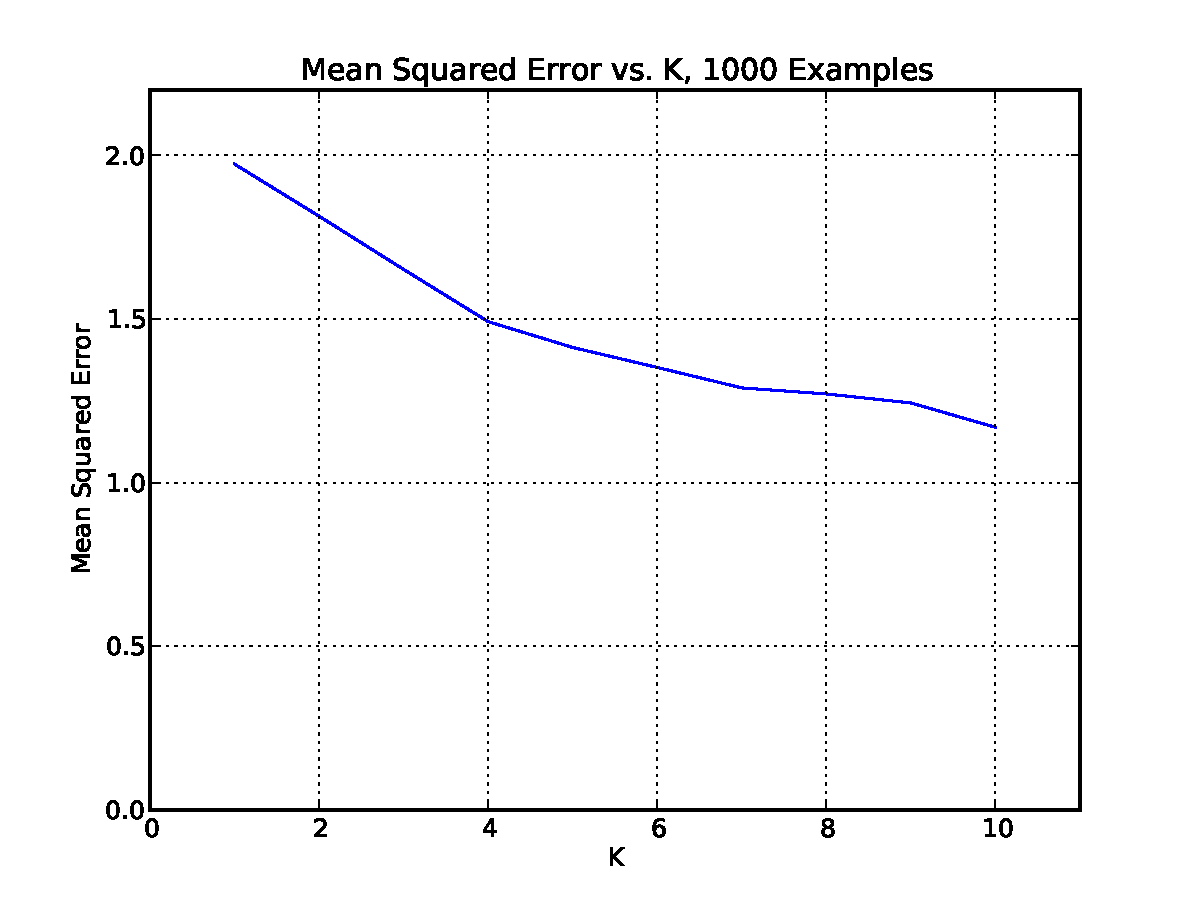
\includegraphics[scale=0.8]{mse-vs-k.pdf}
				\end{center}
			\item If we were to choose the best $K$ for this data based on the plot we generated above, we would choose $K = 8$, since this value of $K$ has a relatively low mean squared error (MSE) without the risk of overcomplicating the model. Choosing a higher value of $K$ will of course result in a lower MSE, but doing this defeats the purpose of clustering, since we are overfitting to the data. In the extreme case, every example in the data will have its own cluster, and the MSE will be 0, but this model does not generalize well.
		\end{enumerate}
	\item
	\item
\end{enumerate}

\end{document}



